\documentclass[11pt]{article}

\usepackage[letterpaper,landscape,margin=0.6in]{geometry}
\usepackage[T1]{fontenc}
\usepackage{lmodern}
\usepackage{amsmath}
\usepackage{tikz}
\usetikzlibrary{arrows.meta,positioning,shapes.geometric,shapes.multipart}

\pagestyle{empty}
\setlength{\parindent}{0pt}

\definecolor{datasetFill}{RGB}{221,236,214}
\definecolor{datasetStroke}{RGB}{127,167,108}
\definecolor{processFill}{RGB}{251,241,207}
\definecolor{processStroke}{RGB}{217,176,80}
\definecolor{blueFill}{RGB}{219,232,250}
\definecolor{blueStroke}{RGB}{98,138,197}
\definecolor{tealFill}{RGB}{215,235,231}
\definecolor{tealStroke}{RGB}{71,144,129}
\definecolor{warnFill}{RGB}{248,224,224}
\definecolor{warnStroke}{RGB}{181,77,77}
\colorlet{ink}{black!85}

\tikzset{
  >={Latex[length=3mm,width=2mm]},
  arrow/.style={-{Latex[length=3mm,width=2mm]}, draw=ink, line width=0.95pt},
  data/.style={
    cylinder,
    shape aspect=0.35,
    draw=datasetStroke,
    fill=datasetFill,
    line width=1pt,
    minimum width=2.5cm,
    minimum height=3.2cm,
    align=center,
    font=\sffamily\small
  },
  box/.style={
    rounded corners=7pt,
    draw=processStroke,
    fill=processFill,
    line width=0.95pt,
    minimum width=3.8cm,
    minimum height=1.7cm,
    align=center,
    font=\sffamily\small
  },
  bluebox/.style={
    rounded corners=7pt,
    draw=blueStroke,
    fill=blueFill,
    line width=0.95pt,
    minimum width=3.8cm,
    minimum height=1.7cm,
    align=center,
    font=\sffamily\small
  },
  tealbox/.style={
    rounded corners=7pt,
    draw=tealStroke,
    fill=tealFill,
    line width=0.95pt,
    minimum width=3.8cm,
    minimum height=1.7cm,
    align=center,
    font=\sffamily\small
  },
  warnbox/.style={
    rounded corners=7pt,
    draw=warnStroke,
    fill=warnFill,
    line width=0.95pt,
    minimum width=4.2cm,
    minimum height=1.7cm,
    align=center,
    font=\sffamily\small
  },
  studytable/.style={
    rectangle split,
    rectangle split parts=4,
    rectangle split part align={center,center,center,center},
    rounded corners=7pt,
    draw=tealStroke,
    fill=tealFill,
    line width=0.95pt,
    minimum width=5.0cm,
    inner sep=3pt,
    font=\sffamily\small
  },
  note/.style={font=\sffamily\footnotesize, text=black!65, align=center}
}

\newcommand{\DiagramTitle}[1]{%
  \node[font=\sffamily\bfseries\Large, text=ink] at (13.2,7.7) {#1};
}

\begin{document}

% --------------------------------------------------------------------------
% Figure 1
% --------------------------------------------------------------------------
\begin{center}
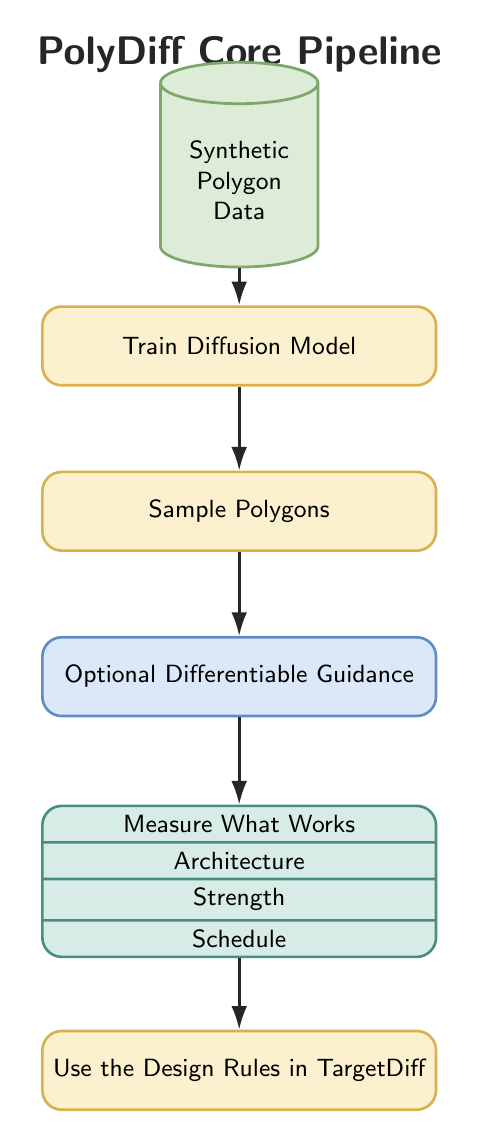
\begin{tikzpicture}[x=1cm,y=1cm]
  \DiagramTitle{PolyDiff Core Pipeline}

  \node[data, shape border rotate=90, minimum width=2.0cm, minimum height=2.6cm] (data) at (13.2,6.1) {Synthetic\\Polygon\\Data};
  \node[box, minimum width=5.0cm, minimum height=1.0cm] (train) at (13.2,4.0) {Train Diffusion Model};
  \node[box, minimum width=5.0cm, minimum height=1.0cm] (sample) at (13.2,1.9) {Sample Polygons};
  \node[bluebox, minimum width=5.0cm, minimum height=1.0cm] (guide) at (13.2,-0.2) {Optional Differentiable Guidance};
  \node[studytable] (study) at (13.2,-2.8) {Measure What Works\nodepart{second}Architecture\nodepart{third}Strength\nodepart{fourth}Schedule};
  \node[box, minimum width=5.0cm, minimum height=1.0cm] (targetdiff) at (13.2,-5.2) {Use the Design Rules in TargetDiff};

  \draw[arrow] (data.south) -- (train.north);
  \draw[arrow] (train.south) -- (sample.north);
  \draw[arrow] (sample.south) -- (guide.north);
  \draw[arrow] (guide.south) -- (study.north);
  \draw[arrow] (study.south) -- (targetdiff.north);
\end{tikzpicture}
\end{center}
\newpage

% --------------------------------------------------------------------------
% Figure 2
% --------------------------------------------------------------------------
\begin{center}
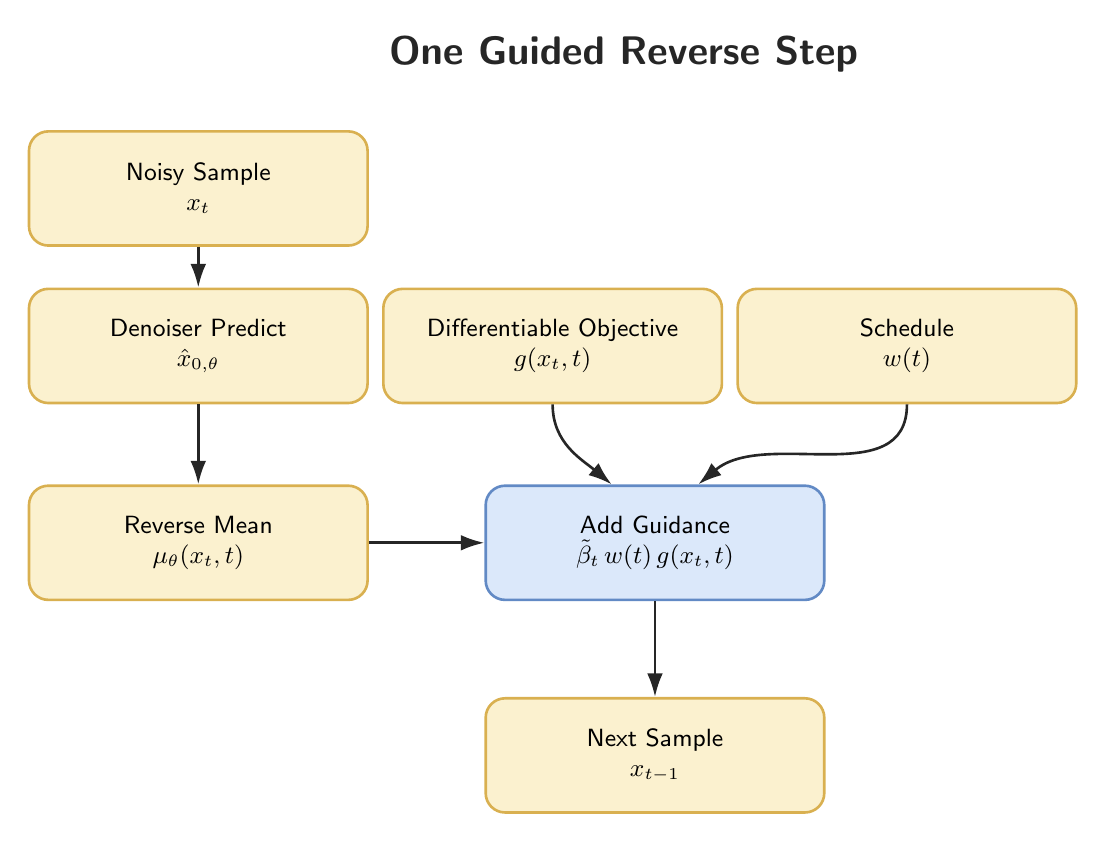
\begin{tikzpicture}[x=1cm,y=1cm]
  \DiagramTitle{One Guided Reverse Step}

  \node[box, minimum width=4.3cm, minimum height=1.45cm] (xt) at (7.8,6.0) {Noisy Sample\\$x_t$};
  \node[box, minimum width=4.3cm, minimum height=1.45cm] (denoiser) at (7.8,4.0) {Denoiser Predict\\$\hat{x}_{0,\theta}$};
  \node[box, minimum width=4.3cm, minimum height=1.45cm] (mean) at (7.8,1.5) {Reverse Mean\\$\mu_\theta(x_t,t)$};

  \node[box, minimum width=4.3cm, minimum height=1.45cm] (objective) at (12.3,4.0) {Differentiable Objective\\$g(x_t,t)$};
  \node[box, minimum width=4.3cm, minimum height=1.45cm] (schedule) at (16.8,4.0) {Schedule\\$w(t)$};

  \node[bluebox, minimum width=4.3cm, minimum height=1.45cm] (guidance) at (13.6,1.5) {Add Guidance\\$\tilde{\beta}_t\,w(t)\,g(x_t,t)$};
  \node[box, minimum width=4.3cm, minimum height=1.45cm] (next) at (13.6,-1.2) {Next Sample\\$x_{t-1}$};

  \draw[arrow] (xt.south) -- (denoiser.north);
  \draw[arrow] (denoiser.south) -- (mean.north);
  \draw[arrow] (mean.east) -- (guidance.west);
  \draw[arrow] (objective.south) to[out=-90,in=140] ([xshift=-0.55cm]guidance.north);
  \draw[arrow] (schedule.south) to[out=-90,in=40] ([xshift=0.55cm]guidance.north);
  \draw[arrow] (guidance.south) -- (next.north);
\end{tikzpicture}
\end{center}
\newpage

% --------------------------------------------------------------------------
% Figure 3
% --------------------------------------------------------------------------
\begin{center}
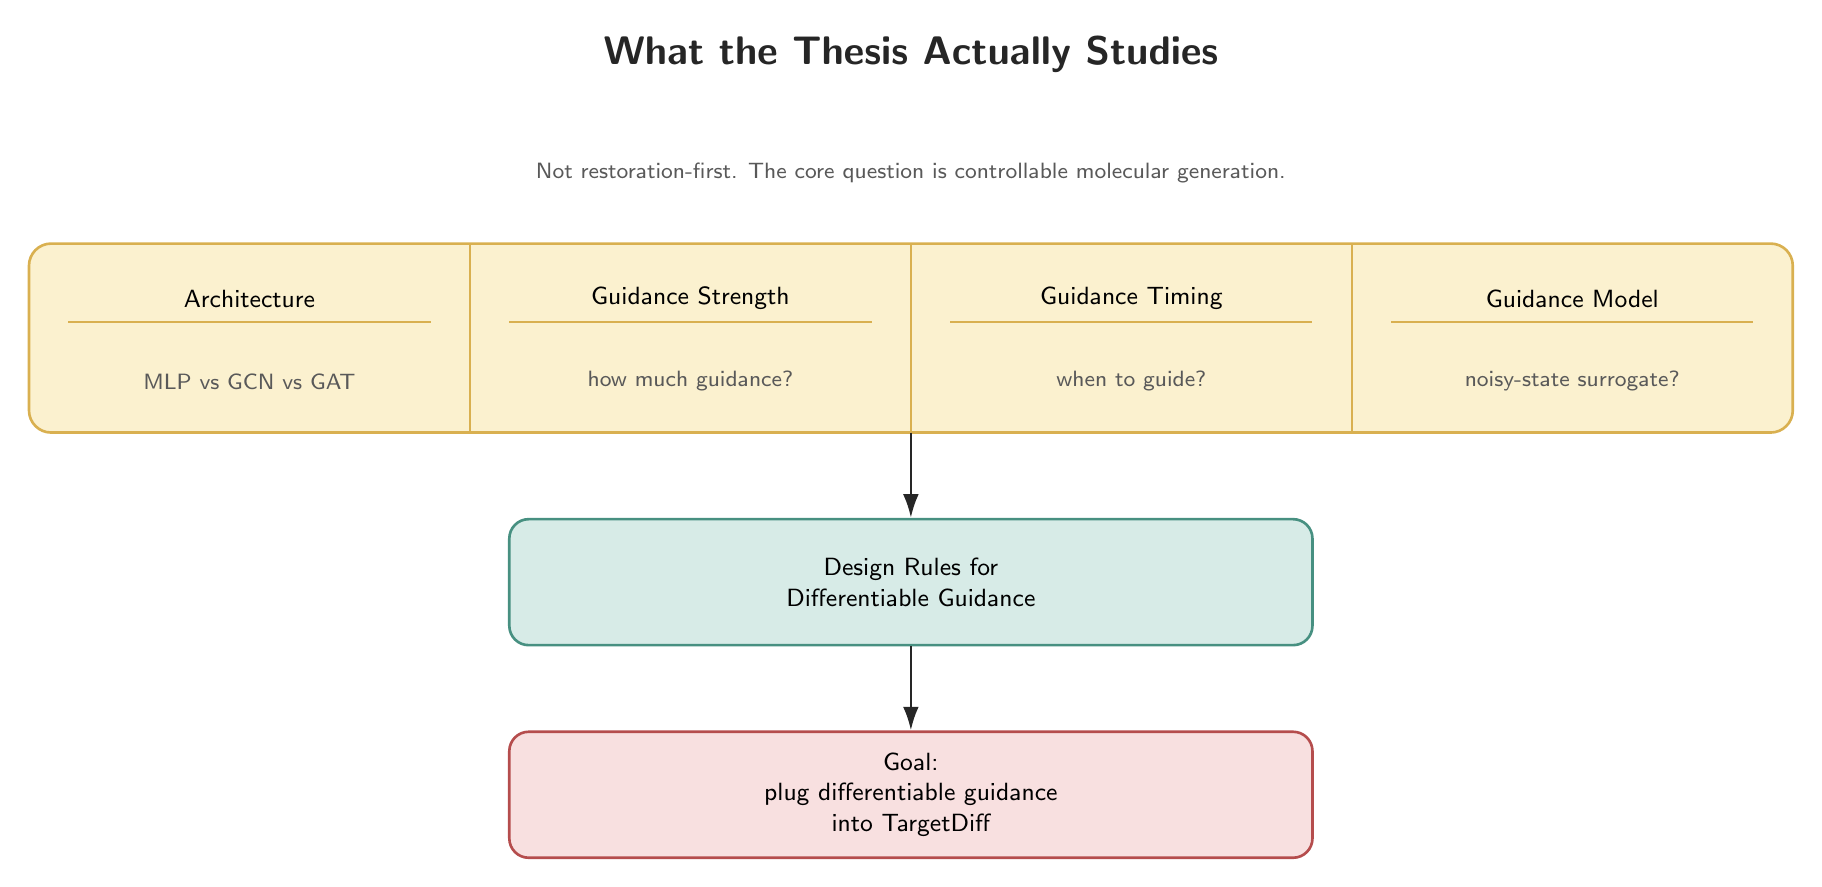
\begin{tikzpicture}[x=1cm,y=1cm]
  \DiagramTitle{What the Thesis Actually Studies}

  \filldraw[rounded corners=8pt, draw=processStroke, fill=processFill, line width=0.95pt]
    (2.0,5.3) rectangle (24.4,2.9);
  \draw[processStroke, line width=0.95pt] (7.6,2.9) -- (7.6,5.3);
  \draw[processStroke, line width=0.95pt] (13.2,2.9) -- (13.2,5.3);
  \draw[processStroke, line width=0.95pt] (18.8,2.9) -- (18.8,5.3);

  \node[font=\sffamily\small, align=center] at (4.8,4.6) {Architecture};
  \draw[processStroke, line width=0.8pt] (2.5,4.3) -- (7.1,4.3);
  \node[note] at (4.8,3.55) {MLP vs GCN vs GAT};

  \node[font=\sffamily\small, align=center] at (10.4,4.6) {Guidance Strength};
  \draw[processStroke, line width=0.8pt] (8.1,4.3) -- (12.7,4.3);
  \node[note] at (10.4,3.55) {how much guidance?};

  \node[font=\sffamily\small, align=center] at (16.0,4.6) {Guidance Timing};
  \draw[processStroke, line width=0.8pt] (13.7,4.3) -- (18.3,4.3);
  \node[note] at (16.0,3.55) {when to guide?};

  \node[font=\sffamily\small, align=center] at (21.6,4.6) {Guidance Model};
  \draw[processStroke, line width=0.8pt] (19.3,4.3) -- (23.9,4.3);
  \node[note] at (21.6,3.55) {noisy-state surrogate?};

  \node[tealbox, minimum width=10.2cm, minimum height=1.6cm] (rules) at (13.2,1.0) {Design Rules for\\Differentiable Guidance};
  \node[warnbox, minimum width=10.2cm, minimum height=1.6cm] (goal) at (13.2,-1.7) {Goal:\\plug differentiable guidance\\into TargetDiff};

  \draw[arrow] (13.2,2.9) -- (rules.north);
  \draw[arrow] (rules.south) -- (goal.north);

  \node[note] at (13.2,6.2) {Not restoration-first. The core question is controllable molecular generation.};
\end{tikzpicture}
\end{center}

\end{document}
